\subsubsection{UC18 - Verifica esistenza funzione}
\begin{figure}[h]
	\centering
	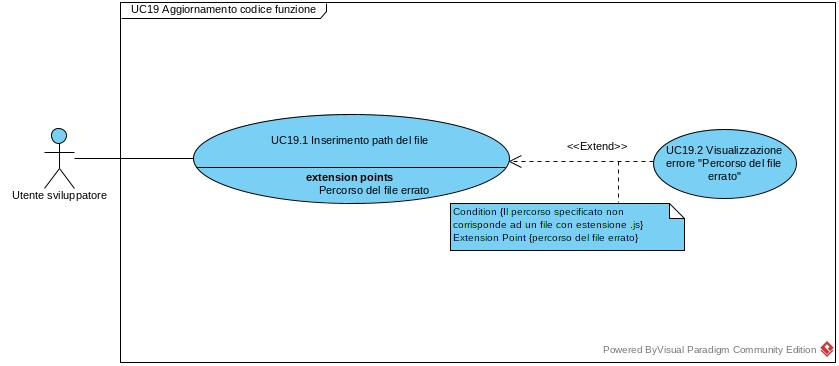
\includegraphics[width=\linewidth]{res/img/UC18.jpg}
	\caption{Diagramma UC18 - Verifica esistenza funzione}
\end{figure}
\begin{itemize}
	\item \textbf{Attori primari:} Utente sviluppatore;
	\item \textbf{Descrizione:} l'utente potrà verificare la presenza di una delle sue funzioni su \textit{Etherless} durante la sua rimozione o la modifica delle impostazioni; 
	\item \textbf{Pre-condizioni:} l'utente ha eseguito il \textit{"deploy\glos"} di almeno una funzione su \textit{Etherless};
	\item \textbf{Post-condizioni:} viene cercata una funzione con nome corrispondente per poter procedere alla sua rimozione o alla modifica dei suoi settaggi;
	\item \textbf{Scenario principale:} 
	\begin{enumerate}
		\item L'utente verifica la presenza di una sua funzione in \textit{Etherless} mediante il comando "find";
		\item Il sistema procederà con l'eliminazione, la modifica dei settaggi o l'update del codice di una funzione a seconda del comando scelto dall'utente.
	\end{enumerate}
\end{itemize}